\documentclass[11pt]{article}
\usepackage{amssymb, amsthm, amsmath}
\usepackage{bm}
\usepackage{graphicx}
\usepackage[authoryear]{natbib}
\usepackage{bm}
\usepackage{verbatim}
\usepackage{lineno}
\usepackage{times}
\usepackage{soul}
\usepackage{color}
\usepackage{enumitem}
\usepackage{setspace}
\usepackage{times}
\usepackage{changepage}
\usepackage{multirow}

\usepackage[left=1in,top=1in,right=1in]{geometry}
\pdfpageheight 11in
\pdfpagewidth 8.5in
\linespread{2.0}
\newcommand{\btheta}{ \mbox{\boldmath $\theta$}}
\newcommand{\bmu}{ \mbox{\boldmath $\mu$}}
\newcommand{\balpha}{ \mbox{\boldmath $\alpha$}}
\newcommand{\bbeta}{ \mbox{\boldmath $\beta$}}
\newcommand{\bdelta}{ \mbox{\boldmath $\delta$}}
\newcommand{\blambda}{ \mbox{\boldmath $\lambda$}}
\newcommand{\bgamma}{ \mbox{\boldmath $\gamma$}}
\newcommand{\brho}{ \mbox{\boldmath $\rho$}}
\newcommand{\bpsi}{ \mbox{\boldmath $\psi$}}
\newcommand{\bepsilon}{ \mbox{\boldmath $\epsilon$}}
\newcommand{\bomega}{ \mbox{\boldmath $\omega$}}
\newcommand{\bOmega}{ \mbox{\boldmath $\Omega$}}
\newcommand{\bDelta}{ \mbox{\boldmath $\Delta$}}
\newcommand{\bSigma}{ \mbox{\boldmath $\Sigma$}}
\newcommand{\bPsi}{\mbox{\boldmath $\Psi$}}
\newcommand{\bOne}{\mbox{\boldmath $1$}}
\newcommand{\omu}{\overline{\mu}}
\newcommand{\oSigma}{\overline{\Sigma}}
\newcommand{\Yt}{{\tilde Y}}
\newcommand{\bA}{ \mbox{\bf A}}
\newcommand{\bP}{ \mbox{\bf P}}
\newcommand{\bx}{ \mbox{\bf x}}
\newcommand{\bX}{ \mbox{\bf X}}
\newcommand{\bB}{ \mbox{\bf B}}
\newcommand{\bT}{ \mbox{\bf T}}
\newcommand{\bZ}{ \mbox{\bf Z}}
\newcommand{\by}{ \mbox{\bf y}}
\newcommand{\bY}{ \mbox{\bf Y}}
\newcommand{\bz}{ \mbox{\bf z}}
\newcommand{\bh}{ \mbox{\bf h}}
\renewcommand{\bm}{ \mbox{\bf m}}
\newcommand{\br}{ \mbox{\bf r}}
\newcommand{\bt}{ \mbox{\bf t}}
\newcommand{\bk}{\mbox{\bf k}}
\newcommand{\bs}{ \mbox{\bf s}}
\newcommand{\bb}{ \mbox{\bf b}}
\newcommand{\bL}{ \mbox{\bf L}}
\newcommand{\bu}{ \mbox{\bf u}}
\newcommand{\bv}{ \mbox{\bf v}}
\newcommand{\bV}{ \mbox{\bf V}}
\newcommand{\bW}{ \mbox{\bf W}}
\newcommand{\bG}{ \mbox{\bf G}}
\newcommand{\bH}{ \mbox{\bf H}}
\newcommand{\bw}{ \mbox{\bf w}}
\newcommand{\bo}{ \mbox{\bf o}}
\newcommand{\bfe}{ \mbox{\bf e}}
\newcommand{\iid}{\stackrel{iid}{\sim}}
\newcommand{\ind}{\stackrel{ind}{\sim}}
\newcommand{\dd}{\; \text{d} }
\newcommand{\ddd}{\text{d} }
\newcommand{\indep}{\stackrel{indep}{\sim}}
\newcommand{\converged}{\stackrel{d}{\rightarrow}}
\newcommand{\goesto}[1]{\stackrel[#1]{}{\longrightarrow}}
\newcommand{\calR}{{\cal R}}
\newcommand{\calG}{{\cal G}}
\newcommand{\calD}{{\cal D}}
\newcommand{\calS}{{\cal S}}
\newcommand{\calB}{{\cal B}}
\newcommand{\calA}{{\cal A}}
\newcommand{\calT}{{\cal T}}
\newcommand{\calO}{{\cal O}}
\newcommand{\argmax}{{\mathop{\rm arg\, max}}}
\newcommand{\argmin}{{\mathop{\rm arg\, min}}}
\newcommand{\Frechet}{\mbox{Fr$\acute{\mbox{e}}$chet }}
\newcommand{\Matern}{\mbox{Mat$\acute{\mbox{e}}$rn }}
\newcommand{\ballunion}{B_a(\bs_1) \cup B_b(\bs_2) }

\newcommand{\alphahat}{\hat{\alpha}}

\newcommand{\eref}[1]{(\ref{#1})}
\newcommand{\fref}[1]{Figure~\ref{#1}}
\newcommand{\tref}[1]{Table~\ref{#1}}
\newcommand{\sref}[1]{Section~\ref{#1}}
\newcommand{\aref}[1]{Appendix~\ref{#1}}

\newcommand{\beq}{ \begin{equation}}
\newcommand{\eeq}{ \end{equation}}
\newcommand{\beqn}{ \begin{eqnarray}}
\newcommand{\eeqn}{ \end{eqnarray}}

\newcommand*\patchAmsMathEnvironmentForLineno[1]{%
  \expandafter\let\csname old#1\expandafter\endcsname\csname #1\endcsname
  \expandafter\let\csname oldend#1\expandafter\endcsname\csname end#1\endcsname
  \renewenvironment{#1}%
     {\linenomath\csname old#1\endcsname}%
     {\csname oldend#1\endcsname\endlinenomath}}% 
\newcommand*\patchBothAmsMathEnvironmentsForLineno[1]{%
  \patchAmsMathEnvironmentForLineno{#1}%
  \patchAmsMathEnvironmentForLineno{#1*}}%
\AtBeginDocument{%
\patchBothAmsMathEnvironmentsForLineno{equation}%
\patchBothAmsMathEnvironmentsForLineno{align}%
\patchBothAmsMathEnvironmentsForLineno{flalign}%
\patchBothAmsMathEnvironmentsForLineno{alignat}%
\patchBothAmsMathEnvironmentsForLineno{gather}%
\patchBothAmsMathEnvironmentsForLineno{multline}%
}



\begin{document}\linenumbers
\pagestyle{empty}
\begin{center}
{\Large {\bf PCA for extremes}}\\

{\large Sam Morris\footnote[1]{North Carolina State University}, Brian J Reich\footnotemark[1]{}, Emeric Thibauld\footnote[2]{Colorado State University}, and Dan Cooley\footnotemark[2]{}}

%\footnote{This is the footnote} looks like this. Later text referring to same footnote\footnotemark[\value{footnote}]
\today
\end{center}


\begin{abstract}
	words...\\
	{\bf Key words}: Max-stable process.

\end{abstract}
\newpage
\pagestyle{plain}
\setcounter{page}{1}

\section{Introduction}\label{s:intro}

\section{Model}\label{s:model}

Let $Y_{t}(\bs)$ be the observation at spatial location $\bs$ and time $t$.  We temporarily drop the subscript $t$ and describe the model for the process $Y(\bs)$ for a single time point, but return to the spatiotemporal setting in Section \ref{s:estimation}.  To focus attention on the extreme values, we emphasize the statistical model for exceedances above a location-specific threshold $T(\bs)$.  We begin by specifying a spatial model for the complete data $Y(\bs)$ and then use the censored likelihood defined by $T(\bs)$ for inference as described in Section \ref{s:MCMC}.


Spatial dependence is captured by modeling $Y(\bs)$ as a max-stable process (ref). Max-stable processes have generalized extremal value (GEV; see Appendix A.1) marginal distribution.  The GEV has three parameters: location $\mu(\bs)$; scale $\sigma(\bs)$; and shape $\xi(\bs)$. Spatial dependence is described for the standardized process
\beq\label{Y2Z}
 Z(\bs) = \left\{1+\frac{\xi(\bs)}{\sigma(\bs)}\left[Y(\bs) - \mu(\bs)\right]\right\}^{1/\xi(\bs)},
\eeq which has unit $\Frechet$ (i.e., GEV with location, scale, and shape all equal one) marginal distribution for all $\bs$.


Our objective is to identify a low-rank model for the spatial dependence of the $Z(\bs)$.   The spectral representation theorem (ref) states that any max-stable process can be written
\beq\label{spectral}
  Z(\bs) = \mbox{sup}_l B(\bs,\bt_l)A_{l}
\eeq
where the function $B$ satisfies $B(\bs,\bt)>0$ for all $(\bs,\bt)$ and $\int B(\bs,\bt)d\bt=1$ for all $\bs$, and $(\bt_l,A_l)$ for $l=1,...,\infty$ are a Poisson process with intensity measure $dA d\bt/A^2$.    This representation provides a means of truncation.  Ref propose the max-linear model
\beq\label{spectral}
Z(\bs) = \bigvee_{l=1}^L B_{l}(\bs)A_l
\eeq
where $B_{l}(\bs)>0$, $\int B_l(\bs)d\bs=1$ for all $L$, and $A_l$ are independent $\Frechet$ random variables.


The assumption that $Z(\bs)$ equals exactly the maximum of a small number of functions is unrealistic, especially for data measured with error.  We therefore follow the Reich and Shaby (ref) and decompose  $Z(\bs)$ as $Z(\bs)=\theta(\bs)\varepsilon(\bs)$ where $\theta(\bs)$ is a spatial process and $\varepsilon(\bs)\iid$ GEV$(1,\alpha,\alpha)$ is independent error.  The spatial component is
\beq \label{theta}
  \theta(\bs) = \left(\sum_{l=1}^LB_{l}(\bs)^{1/\alpha}A_{l}\right)^{\alpha}.
\eeq
If $B_{l}(\bs)>0$, $\sum_{l=1}^LB_{l}(\bs)=1$ for all $\bs$, and the $A_{l}$ have positive stable (PS; Appendix A.1) distribution $A_{l}\iid$ PS$(\alpha)$, then $Z(\bs)$ is max-stable and has unit $\Frechet$ marginal distributions.

Extremal spatial dependence can be summarized by the extremal coefficient (EC; ref) $\vartheta(\bs,\bt)\in[1,2]$, where
\beq\label{ECdev}
  \mbox{Prob}[Z(\bs)<c,Z(\bt)<c] = \mbox{Prob}[Z(\bs)<c]^{\vartheta(\bs,\bt)}.
\eeq
For the PS random effects model the EC has the form
\beq\label{EC}
   \vartheta(\bs,\bt) = \sum_{l=1}^L \left[B_{l}(\bs)^{1/\alpha}+B_{l}(\bs)^{1/\alpha}\right]^\alpha.
\eeq
In particular, $\vartheta(\bs,\bs) = 2^{\alpha}$ for all $\bs$.

\section{Estimating the spatial dependence function}\label{s:estimation}

To estimate the extremal coefficient function, we consider the process at $n_s$ spatial locations $\bs_1,...,\bs_{n_s}$ and $n_t$ times $t=1,...,n_t$.  Denote $Y_t(\bs_i) = Y_{it}$, $B_l(\bs_i) = B_{il}$, $T(\bs_i)=T_i$, and $\vartheta(\bs_i,\bs_j) = \vartheta_{ij}$.  In this section we develop an algorithm to estimate the spatial dependence parameter $\alpha$ and the $n_s\times L$ matrix $\bB = \{B_{il}\}$.  Given these parameters, we insert them into our model and proceed with Bayesian analysis as described in Section \ref{s:MCMC}.  Our algorithm has the following steps:
\begin{itemize}
  \item[] (1) Obtain an initial estimate of the extremal coefficient for each pair of locations, ${\hat \vartheta}_{ij}$.
  \item[] (2) Spatially smooth these initial estimates ${\hat \vartheta}_{ij}$ using kernel smoothing to obtain ${\tilde \vartheta}_{ij}$.
  \item[] (3) Estimate the spatial dependence parameters by minimizing the difference between model-based coefficients, $\vartheta_{ij}$, and smoothed coefficients, ${\tilde \vartheta}_{ij}$.
\end{itemize}

The first-stage estimates are obtained using the approach of XXX.  To estimate the spatial dependence we first remove variation in the marginal distribution.  Let $U_{it} = \sum_{k=1}^{n_t} I[Y_{ik}<Y_{it}]/n_t$, so that the $U_{it}$ are approximately uniform at each location.  Then for some extreme probability $q\in(0,1)$, solving (\ref{ECdev}) suggests the estimate
\beq\label{EChat0}
   {\hat \vartheta}_{ij}(q) = \frac{\log[Q_{ij}(q)]}{\log(q)},
\eeq
where $Q_{ij}(q) = \sum_{t=1}^{n_t}I[U_{it}<q,U_{jt}<q]/n_t$ is the sample proportion of the time points at which both sites are less than $q$.  Since all large $q$ give valid estimates, we average over a grid of $q$ with $q_1<...<q_{n_q}$
\beq\label{EChat1}
{\hat \vartheta}_{ij} = \frac{1}{n_q}\sum_{j=1}^{n_q}{\hat \vartheta}_{ij}(q_j).
\eeq

Assuming the true EC is smooth over space, the initial estimates ${\hat \vartheta}_{ij}$ can be improved by smoothing.  Let
\beq\label{EChat2}
  {\tilde \vartheta}_{ij} = \frac{\sum_{u=1}^{n_s}\sum_{v=1}^{n_s} w_{iu}w_{jv}{\hat \vartheta}_{uv}}
  {\sum_{u=1}^{n_s}\sum_{v=1}^{n_s} w_{iu}w_{jv}},
\eeq
where $w_{iu} = \exp[-(||\bs_i-\bs_u'||/\phi)^2])$ is the Gaussian kernel function with bandwidth $\phi$.  The elements ${\hat \vartheta}_{ii}$ do not contribute any information as ${\hat \vartheta}_{ii}=1$ for all $i$ by construction.  To eliminate the influence of these estimates we set $w_{ii}=0$.  However, this approach does give imputed values ${\tilde \vartheta}_{ii}$, which provide information about small-scale spatial variability.

The dependence parameters are estimated by comparing estimates ${\tilde \vartheta}_{ij}$ with the model-based values $\vartheta_{ij}$.  For all $i$, $\vartheta_{ii} = 2^{\alpha}$, and therefore we set $\alpha$ to $\alphahat = \log_2(\sum_{i=1}^{n_s}{\tilde \vartheta}_{ii}/n_s)$. Given $\alpha=\alphahat$, it remains to estimate $\bB$. The estimate ${\hat \bB}$ is the minimizer of
\beq\label{Bhat}
\sum_{i<j} \left({\tilde \vartheta}_{ij} - \vartheta_{ij}\right)^2
  =
  \sum_{i<j} \left({\tilde \vartheta}_{ji} - \sum_{l=1}^L[B_{il}^{1/\alphahat} + B_{jl}^{1/\alphahat}]^{\alphahat}\right)^2
\eeq
under the restrictions that $B_{il}\ge 0$ for all $i$ and $l$ and $\sum_{l=1}^LB_{il}=1$ for all $i$. Since the minimizer of (\ref{Bhat}) does not have a closed form, we use block coordinate descent to obtain ${\hat \bB}$.  We cycle through spatial locations and update the vectors $(B_{i1},...,B_{iL})$ conditioned on the values for the other location and repeat until convergence.  At each step, we use the restricted optimization routine in the {\tt R} (ref) function {\tt optim}.  This algorithm gives estimates of the $B_{il}$ at the $n_s$ data locations, but is easily extended to all $\bs$ for spatial prediction.  The kernel smoothing step ensures that the estimates for ${\hat B}_{il}$ are spatially smooth, and thus interpolation of the ${\hat B}_{il}$ gives spatial functions ${\hat B}_l(\bs)$.

The relative contribution of each term can be measured by
\beq\label{v}
v_l = \frac{1}{n_s}\sum_{i=1}^{n_s}{\hat B}_{il}.
\eeq
Since $\sum_{l=1}^L{\hat B}_{il}=1$ for all $i$, we have $\sum_{l=1}^Lv_l = 1$.  Therefore, terms with large $v_l$ are the most important.  The order of the terms is arbitrary, and so we reorder the terms so that $v_1\ge...\ge v_L$.

\section{Bayesian implementation details}\label{s:MCMC}
For our data analysis in Section \ref{s:analysis} we allow the GEV location and scale parameters, denoted $\mu_{it}$ and scale $\sigma_{it}$ respectively, to vary with space and time.  The GEV shape parameter $\xi$ is held constant over space and time because this parameter is notoriously difficult to estimate (ref).  Collectively, let the marginal GEV parameters at location $i$ and time $t$ be $\Theta_{it} = \{\mu_{it},\sigma_{it},\xi\}$. The GEV location and scale vary according to covariates $\bX_{it}$ with $\mu_{it} = \bX_{it}^T\bbeta_1$ and
$\mbox{log}(\sigma_{it}) = \bX_{it}^T\bbeta_2$.  For covariates we use the standardized linear time trend $t^* = (t-n_t/2)/n_t$, the estimated functions ${\hat B}_{il}$, and their interactions: $\bX_{it} = (1,t^*,{\hat B}_{i1},...,{\hat B}_{iL},t^*{\hat B}_{i1},...,t^*{\hat B}_{iL})^T$.

As shown in R and S (ref), the uncensored responses $Y_{it}$ are conditionally independent given the spatial random effects, with conditional distribution \beq\label{Ycond}
   Y_{it}|\theta_{it},\Theta_{it}\indep GEV(\mu^*_{it}, \sigma_{it}^*,\xi^*),
\eeq
where $\mu_{it}^* = \mu_{it} + \frac{\sigma_{it}}{\xi}(\theta_{it}^\xi-1)$,
$\sigma_{it}^* = \alpha\sigma_{it}\theta_{it}^\xi$, and $\xi^* = \alpha\xi$.  Therefore, the conditional likelihood conveniently factors across observations; marginalizing over the random effect $\theta_{it}$ induces extremal spatial dependence. To focus on the extreme values above the local threshold $T_i$, we use the censored likelihood
\beq\label{g}
d(y;\theta_{it},\Theta_{it})  =
\left\{\begin{array}{ll}
    F(y;\mu_{it}^*,\sigma_{it}^*,\xi^*) & y \le T_i \\
  f(y;\mu_{it}^*,\sigma_{it}^*,\xi^*) & y>T_i,
\end{array}\right.
\eeq
where $F$ and $f$ are the GEV distribution and density functions, respectively, defined in Appendix A.1.


In summary, given the estimates of $\alpha$ and $\bB$, the hierarchical model is
\beqn \label{bayesmodel}
  Y_{it} |\theta_{ij} & \indep & d(y;\theta_{it},\Theta_{it}) \\
  \theta_{it} &=& \left(\sum_{l=1}^L{\hat B}_{il}^{1/\alphahat}A_{lt}\right)^{\alphahat}
  \mbox{\ \ \ where \ \ \ }
  A_{lt} \iid PS(\alphahat)\nonumber\\
  \mu_{it} &=& \bX_{it}^T\bbeta_1
  \mbox{\ \ \ and \ \ \ }
  \mbox{log}(\sigma_{it}) = \bX_{it}^T\bbeta_2. \nonumber
\eeqn
To complete the Bayesian model, we select independent normal priors with mean zero and variance $\sigma^2_1$ and $\sigma^2_2$ for the components of $\bbeta_1$ and $\bbeta_2$ respectively, and $\xi\sim \mbox{Normal}(0,0.5^2)$.
We use inverse gamma (1, 1) priors for $\sigma^2_1$ and $\sigma^2_2$.
The first-stage estimate of the extremal coefficients has three tuning parameters: the quantile thresholds $q_1,...,q_{n_q}$, the kernel bandwidth $\phi$, and the number of terms $L$.
We set $\{q_1,...,q_{n_q}\} = \{0.95,0.96,...,0.99\}$.  In Section \ref{s:analysis} we explore a few possibilities for $\phi$ and $L$ and discuss sensitivity to these choices.
The second-stage Bayesian analysis requires selecting thresholds $T_i,...,T_{n_s}$.  For this we use spatially smoothed sample quantiles.  That is, we set $T_i$ to the 0.95 quantile of the $Y_{it}$ and $Y_{jt}$ for sites $j$ with $||\bs_i-\bs_j||<r$, where $r$ is set to XXX?

We estimate parameters $\Theta = \left\{A_{lt}, \bbeta_1, \bbeta_2, \xi, \sigma^2_1, \sigma^2_2 \right\}$ using Markov chain Monte Carlo methods.
We use a Metropolis-Hastings algorithm to update the model parameters with random walk candidate distributions for all parameters except $\sigma^2_1, \sigma^2_2$ which we update using Gibbs sampling.
The positive stable density can be challenging to evaluate due to the integral inside the density function.
One technique to avoid this complication is to incorporate auxiliary i.i.d. Uniform(0, 1) random variables (Stephenson et al, \hl{ref}).
We opt for a numerical approximation to the integral using 51 evenly spaced quantiles for a Beta(0.5, 0.5) distribution.

\section{Analysis of extreme Georgia fires}\label{s:analysis}
The dataset used for our application is composed of yearly acreage burned due to wildfires for each county in Georgia from 1965 -- 2014 (\texttt{http://weather.gfc.stat.ga.us/FireData/}).
Figure \ref{fig:firets25} shows the time series of $\log$(acres burned) for 25 randomly selected counties.
Based on this plot, and some other exploratory analysis, we see no evidence of non-linear trends and proceed with linear time trends for the GEV location and scale parameters.

\begin{figure}[htbp]
  \centering
  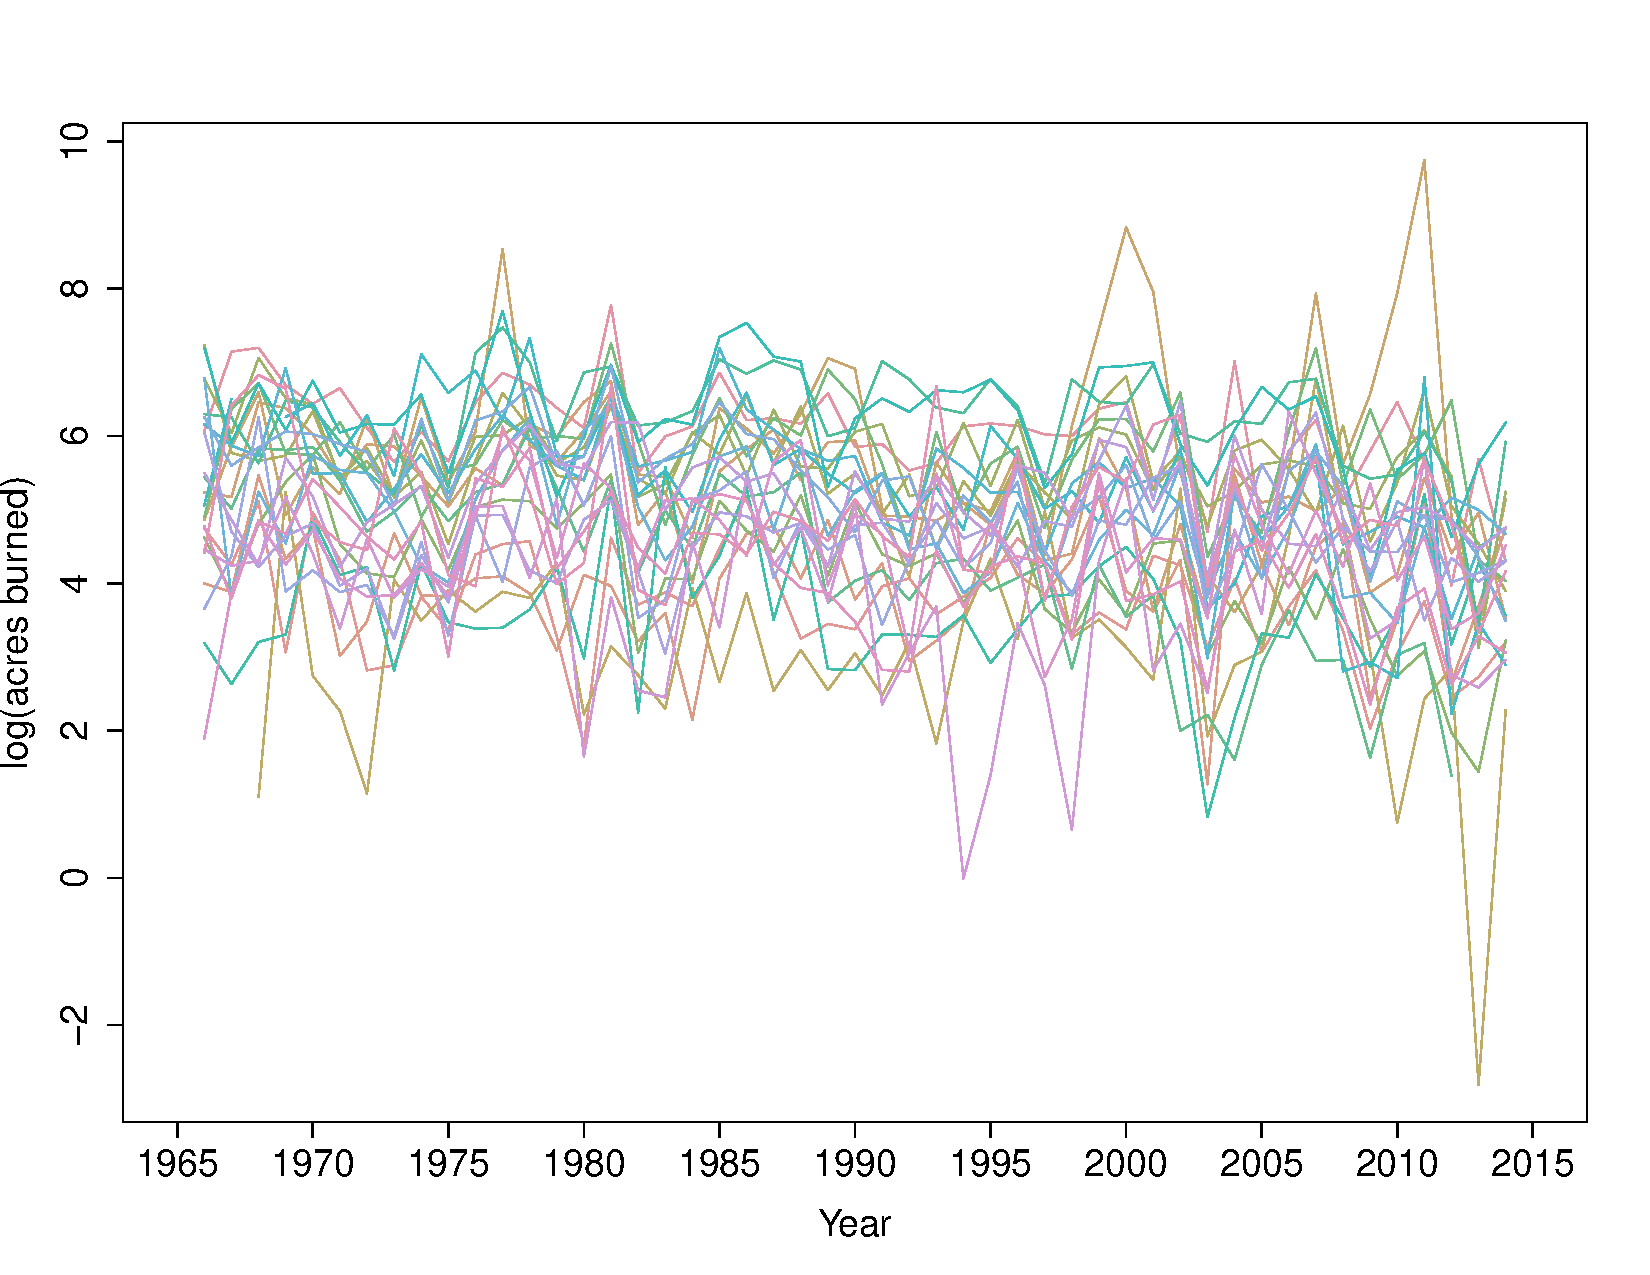
\includegraphics[width=0.80\linewidth]{plots/spag-rand-25}
  \caption{Time series of $\log$(acres burned) for 25 randomly selected counties. \hl{need to change coloring to different region in GA (NE, NW, SE, SW)}}
  \label{fig:firets25}
\end{figure}

We estimate the extremal coefficient function $\hat{\theta}_{ij}$ by setting $q_1 = 0.90$ and using $n_q = 100$.
With more data, it would possible to increase $q_1$, but we set $q_1 = 0.90$ to increase the stability when estimating $\hat{\vartheta}_{ij}$.

Because these data are not max-stable, we select a site-specific threshold $T_i$ to use in the analysis with the following algorithm.
Without some adjustment to the data, it is challenging to borrow information across sites to inform the threshold selection.
We first compute
\begin{align}
  \tilde{\bY}_i = \frac{\bY_i - \text{med}(\bY_i)}{\text{IQR}(\bY_i)}
\end{align}
where med$(\cdot)$ is the median, and IQR$(\cdot)$ is the inter-quartile range.
Then we combine all sites together and plot a mean residual plot for $\tilde{\bY_i}, i = 1, \ldots, n_s$.
The mean residual plot is given in Figure \ref{fig:mrlthresh}, with a vertical line indicating the quantile we use for the county-specific values $\bT$.
Based upon the mean residual plot, we select $q(0.95)$ for the spatially smoothed threshold.
To calculate $T_i$ for each county, we find $\hat{q}(0.95)$ by taking the 95$th$ quantile for county $i$ and the five closest counties.

\begin{figure}[htbp]
  \centering
  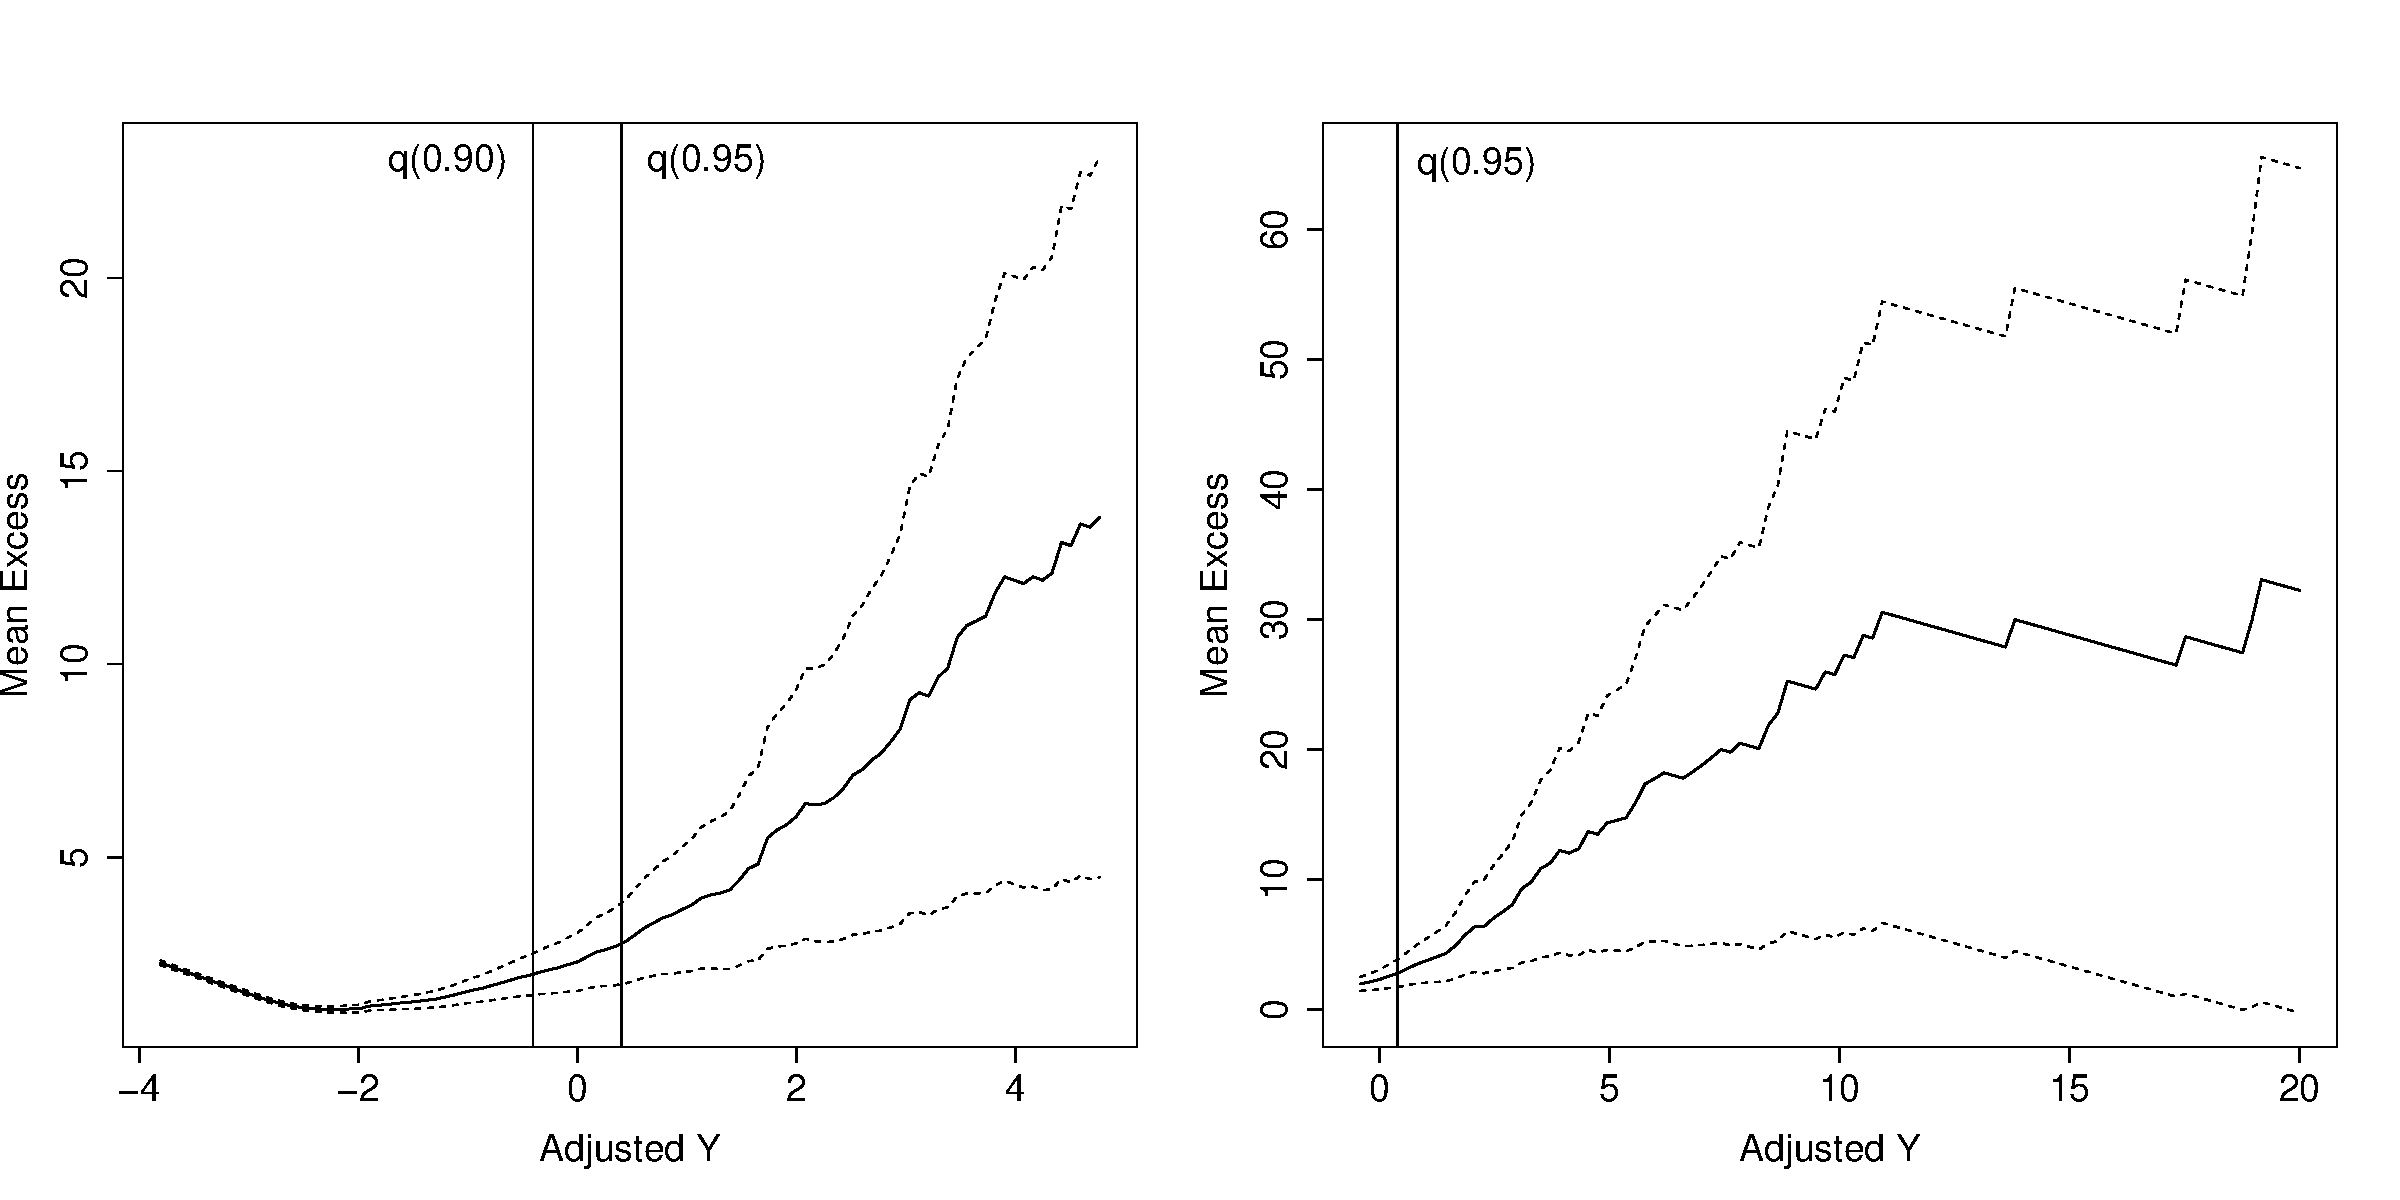
\includegraphics[width = \linewidth]{plots/mrl-plots-fire.pdf}  % markdown/eda/eda-plotting.R
  \caption{Mean residual plot from min(Adj Y) to q(0.995) (left). Mean residual plot from q(0.90) to 20 (right). Vertical lines for q(0.90) and q(0.95) are given in the plots.}
  \label{fig:mrlthresh}
\end{figure}

\begin{figure}[htbp]
  \centering
  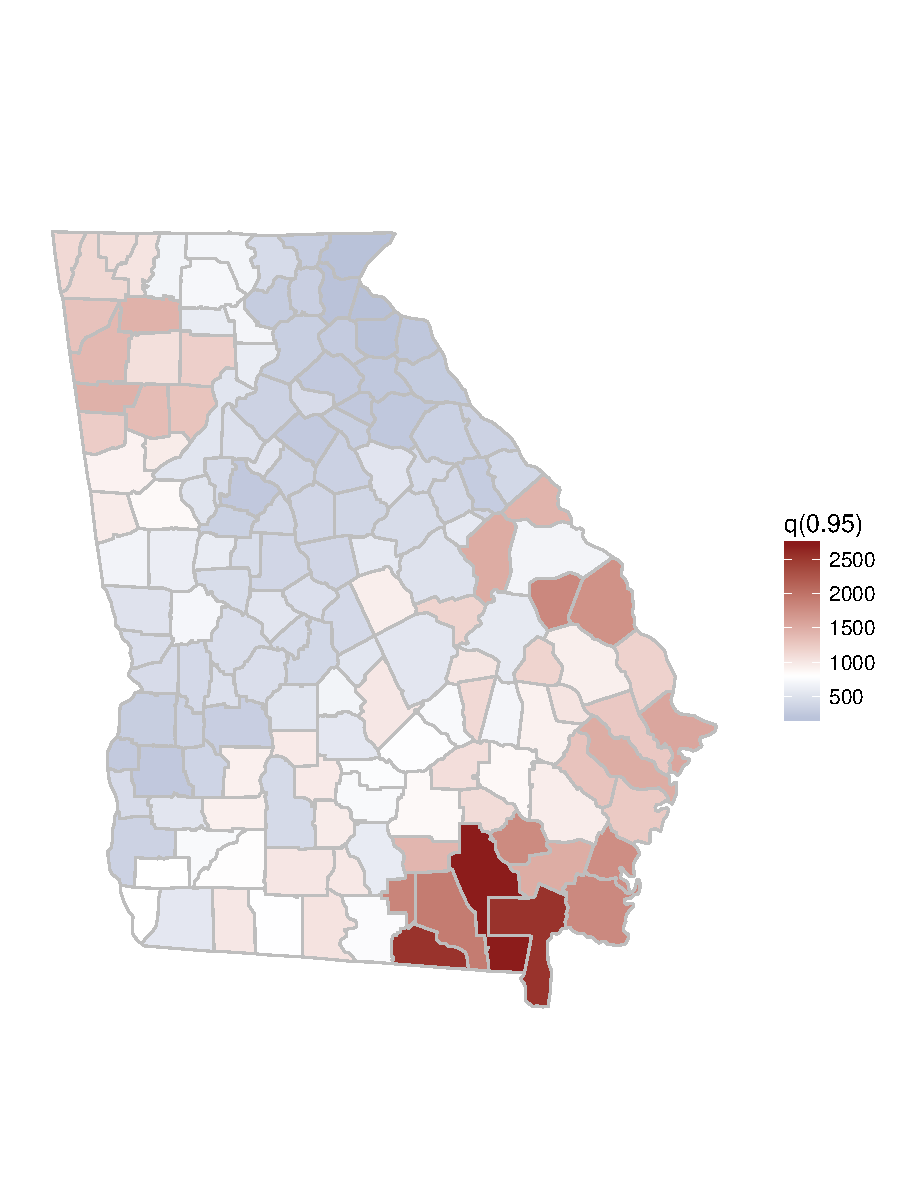
\includegraphics[width = 0.47\linewidth, trim = 0 10em 0 10em]{plots/spatial-q95.pdf}
  \caption{Spatially smoothed threshold values for each county.}
  \label{fig:mrlthresh}
\end{figure}

\subsection{Results}\label{s:results}
We use 10-fold cross-validation to assess the predictive performance of a model.
For each method, we randomly select 90\% of the observations across counties and years to be used as a training set to fit the model.
The remaining 10\% of sites and years are withheld for testing model predictions.
To assess the predictions for the test set, we use quantile scores and Brier scores \hl{citation}.
The quantile score is given by \hl{give formula}.
The Brier score is given by \hl{give formula}.
For both of these methods, we use a negative orientation, so a lower score indicates a better fit.

\begin{table}[htbp]
\caption{Average quantile scores for selected quantiles and Brier scores ($\times 100$) for selected thresholds}
\centering
\small
  \begin{tabular}{lcc|rr|rr}
   \multicolumn{3}{c}{  }& \multicolumn{2}{c|}{Brier Scores ($\times 100$)} & \multicolumn{2}{|c}{Quantile Scores}\\
   \hline
   & Process & Marginal & $q(0.95)$ & $q(0.99)$ & $q(0.95)$ & $q(0.99)$\\
   \hline
  \multirow{4}{*}{L = 5} & ebf & ebf & 6.065 & 2.443 & 159.30 & 90.87 \\
                         & ebf & gsk & 5.622 & 2.221 & 130.46 & 78.33 \\
                         & gsk & ebf & 5.830 & 2.332 & 145.20 & 83.40 \\
                         & gsk & gsk & 5.612 & 2.238 & 129.26 & 76.95 \\
   \hline
  \multirow{4}{*}{L = 10} & ebf & ebf & 5.962 & 2.405 & 147.05 & 84.42 \\
                          & ebf & gsk & 5.299 & 2.160 & 126.18 & 72.64 \\
                          & gsk & ebf & 5.727 & 2.293 & 137.58 & 77.96 \\
                          & gsk & gsk & 5.337 & 2.186 & 128.28 & 74.05 \\
   \hline
  \multirow{4}{*}{L = 15} & ebf & ebf & 5.960 & 2.384 & 149.40 & 84.02 \\
                          & ebf & gsk & 5.172 & 2.114 & 129.48 & 74.85 \\
                          & gsk & ebf & 5.739 & 2.258 & 138.67 & 78.86 \\
                          & gsk & gsk & 5.153 & 2.123 & 130.35 & 74.50 \\
   \hline
  \multirow{4}{*}{L = 20} & ebf & ebf & 5.911 & 2.364 & 170.20 & 97.43 \\
                          & ebf & gsk & 5.177 & 2.109 & \textbf{126.16} & 72.33 \\
                          & gsk & ebf & 5.680 & 2.234 & 139.08 & 78.48 \\
                          & gsk & gsk & \textbf{5.077} & 2.113 & 128.20 & 71.47 \\
   \hline
  \multirow{4}{*}{L = 25} & ebf & ebf & 5.848 & 2.343 & *****  & ***** \\
                          & ebf & gsk & 5.206 & \textbf{2.095} & 127.06 & \textbf{70.53} \\
                          & gsk & ebf & 5.595 & 2.233 & *****  & ***** \\
                          & gsk & gsk & 5.124 & 2.116 & 129.43 & 72.16 \\
  \hline
  L = 159 & gsk & gsk & 5.00 & 2.08 & 127.72 & 68.70 \\
  \hline
	\end{tabular}
\end{table}

\begin{figure}  % markdown/fire-analysis/combine-tables.R
  \centering
  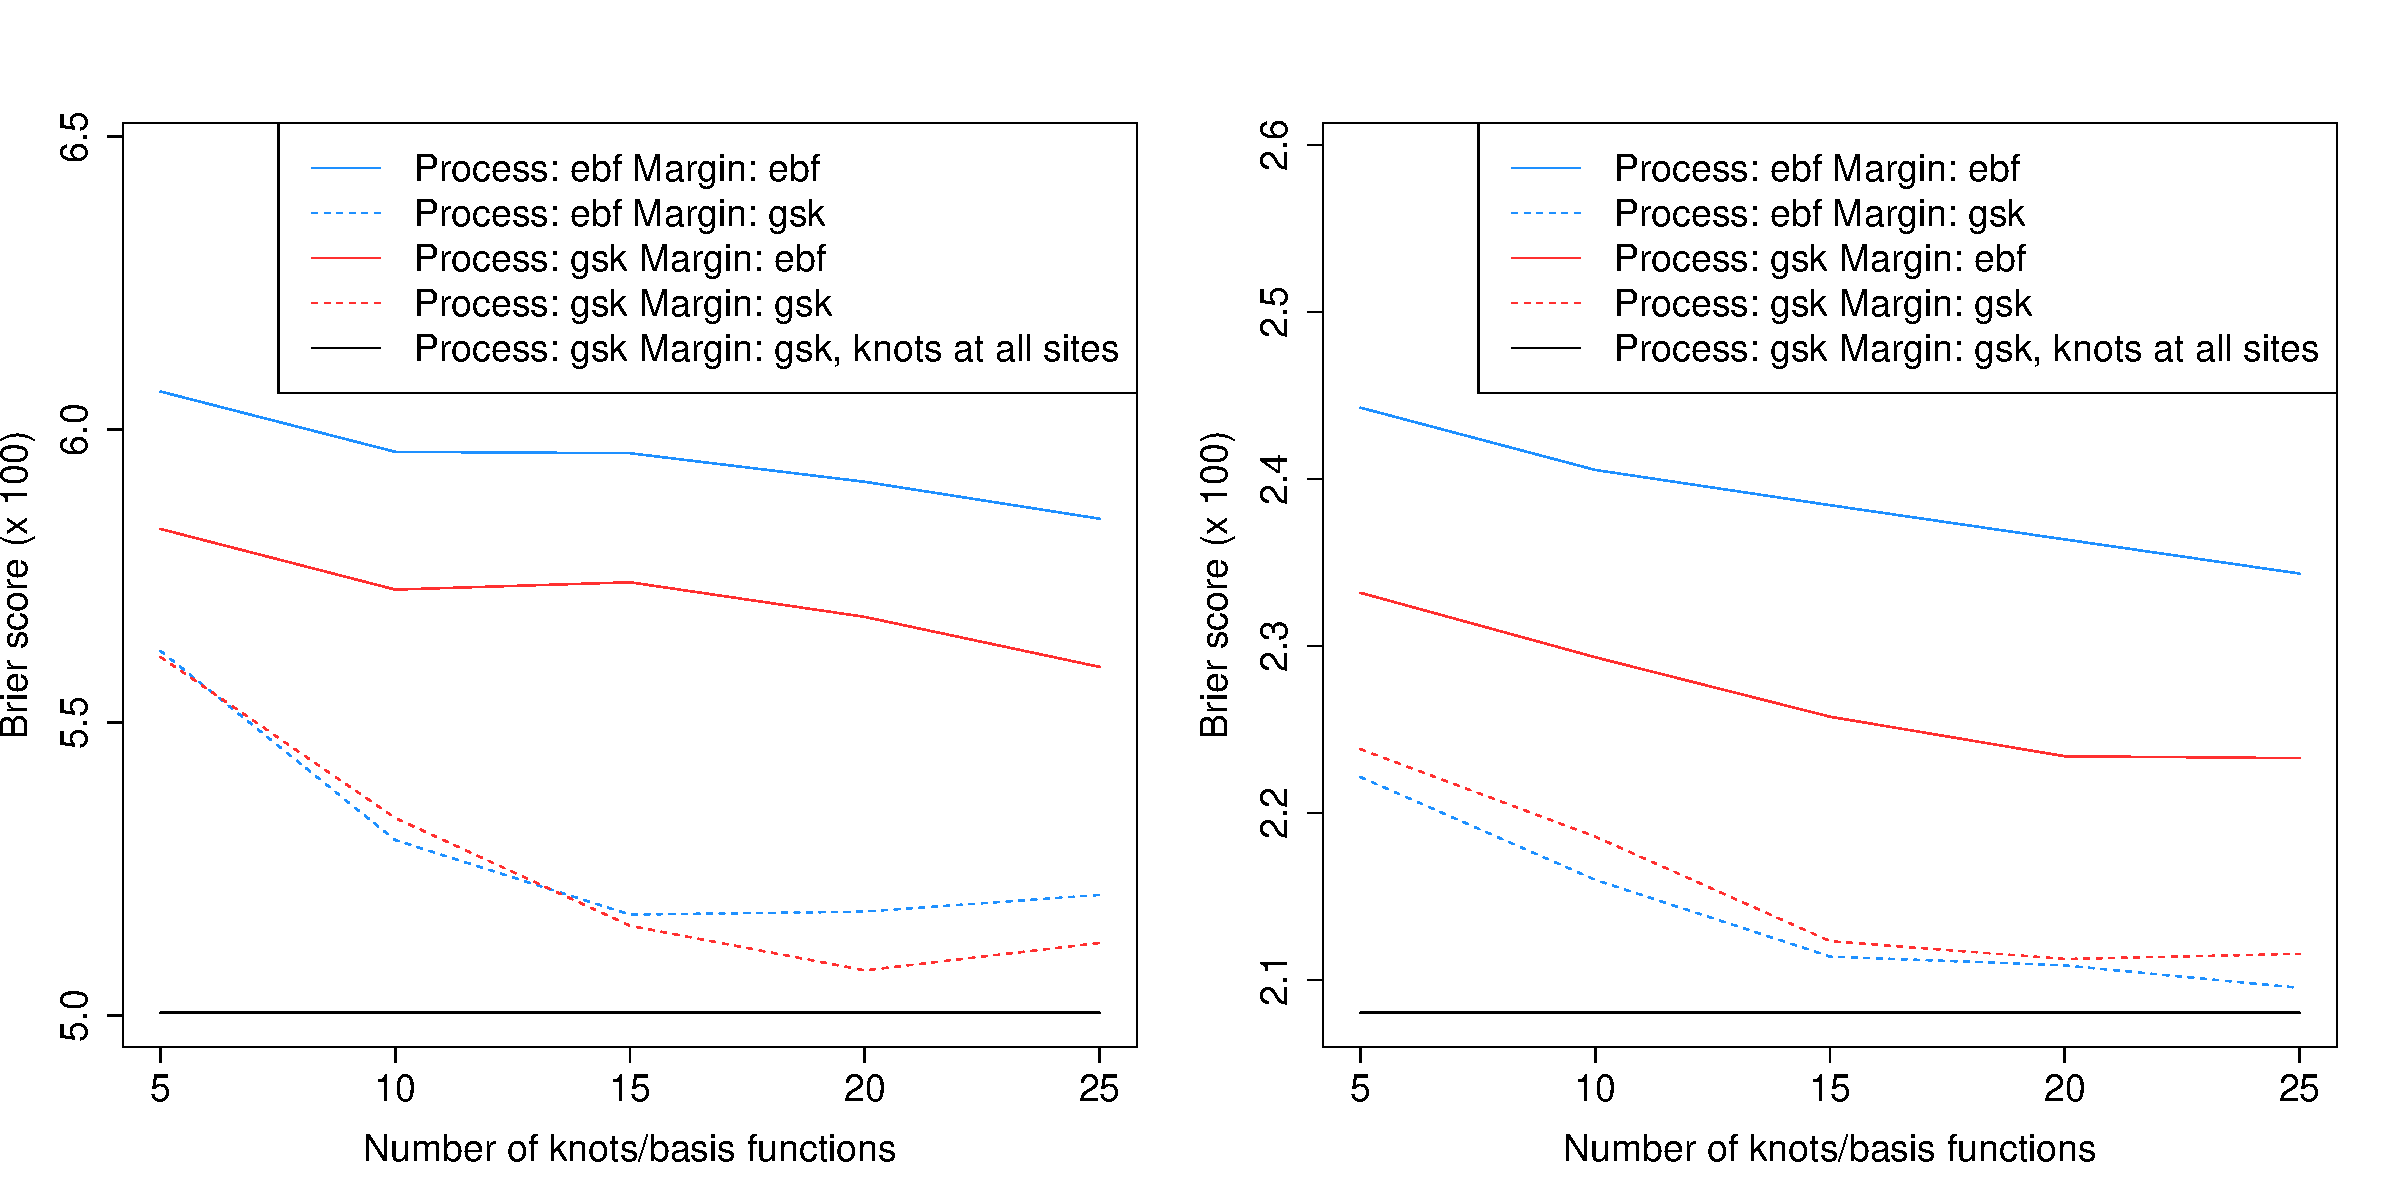
\includegraphics[width=\linewidth]{plots/bs-mean-fire}
  \caption{Average Brier score for exceeding q(0.95) (left). Average Brier score for exceeding q(0.99) (right).}
  \label{fig:avgqscore}
\end{figure}

\begin{figure}  % markdown/fire-analysis/combine-tables.R
	\centering
	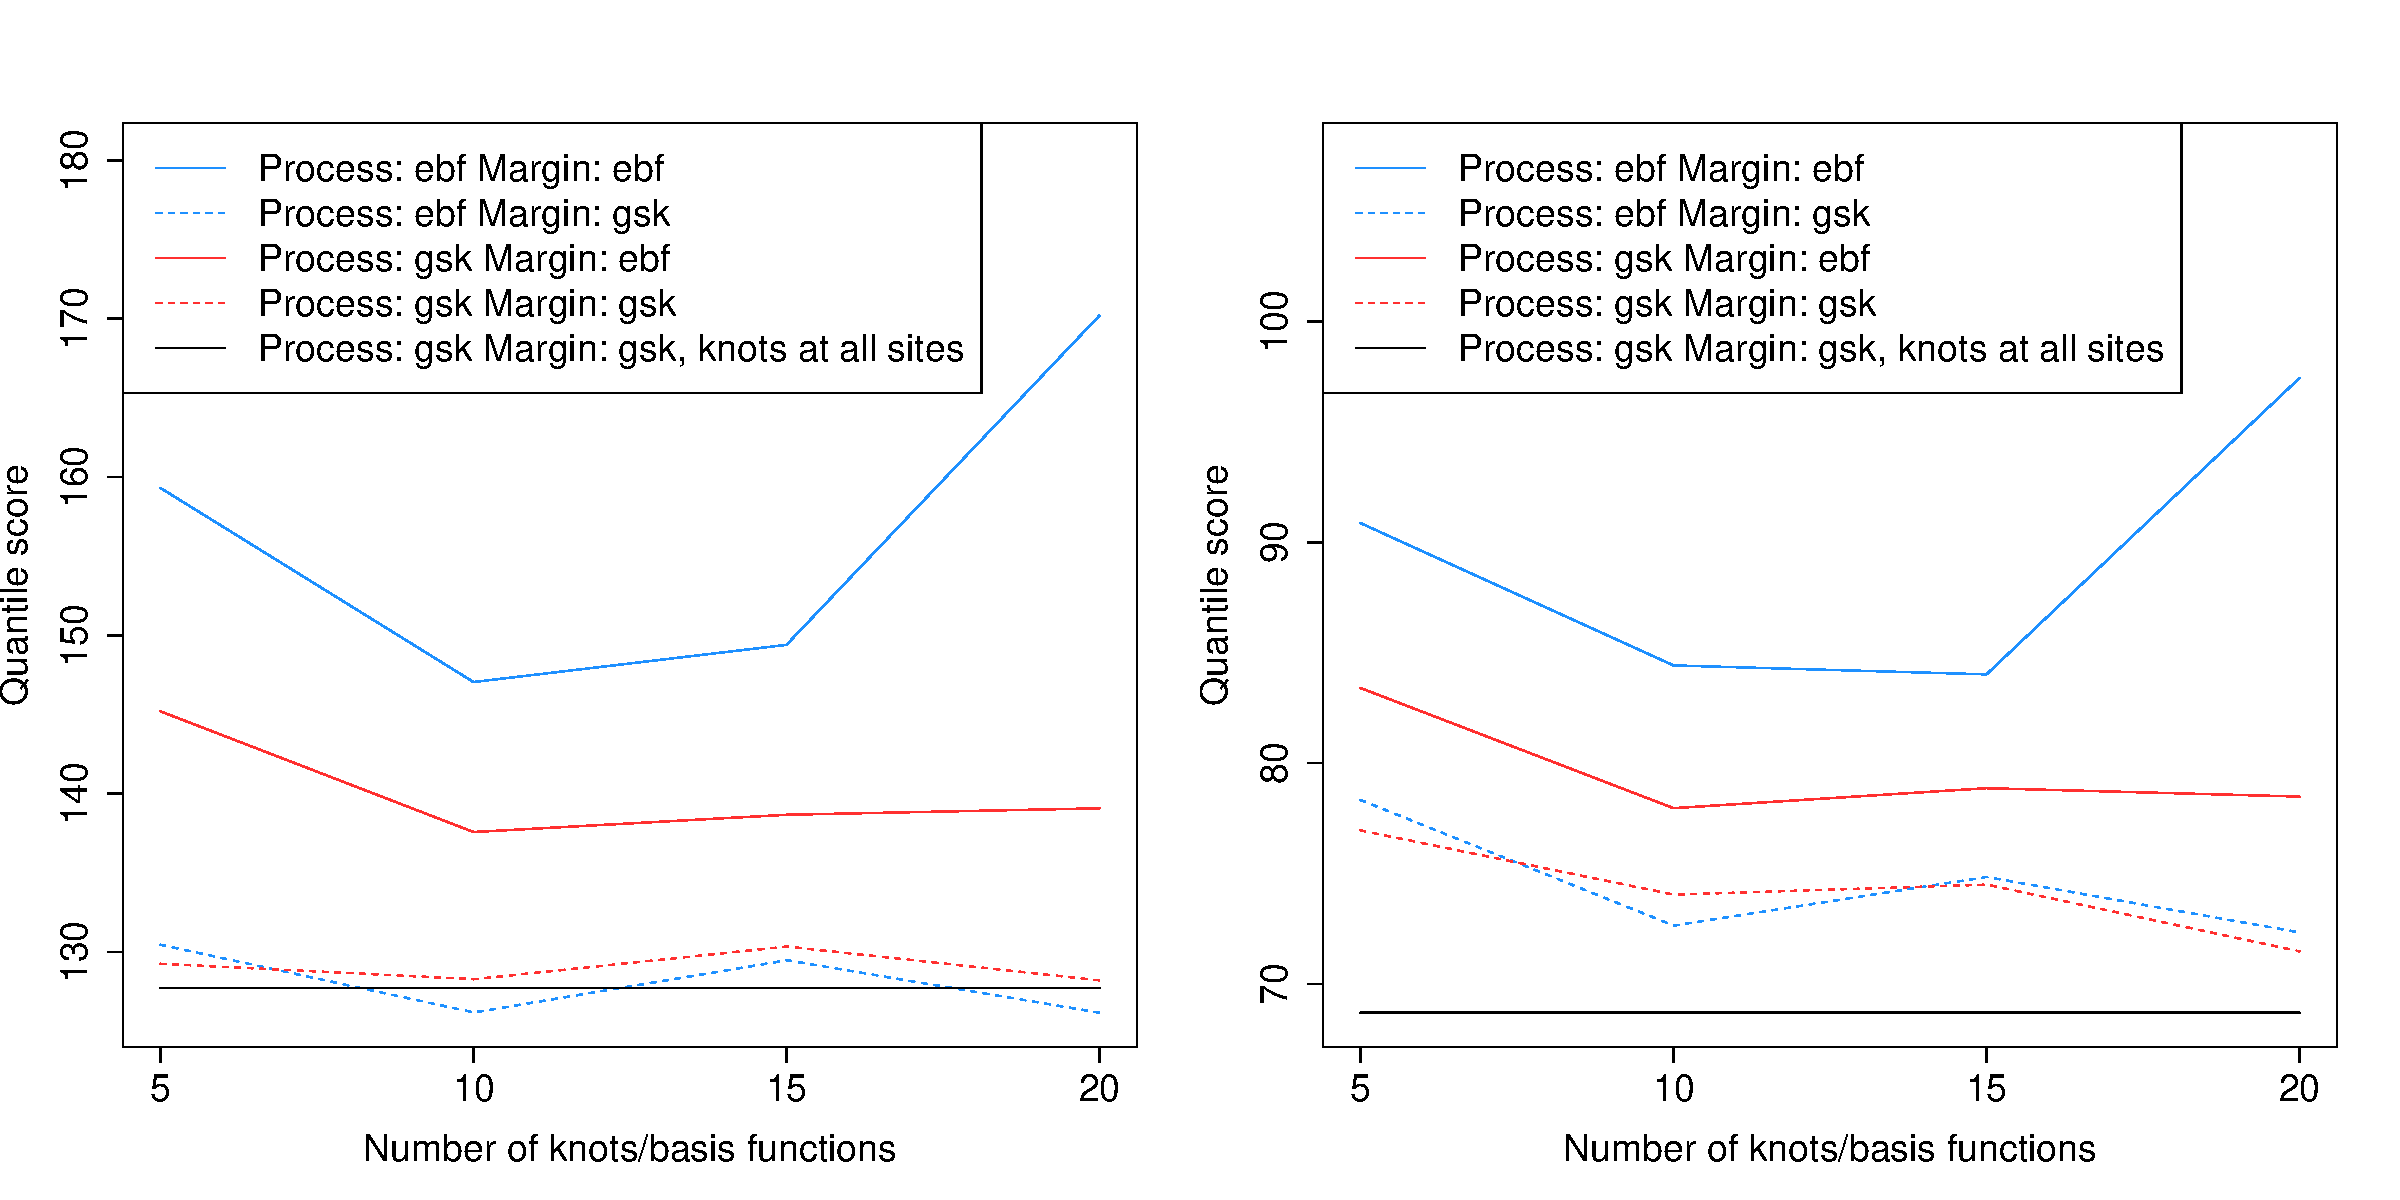
\includegraphics[width=\linewidth]{plots/qs-mean-fire}
	\caption{Average quantile score for q(0.95) (left). Average quantile score for q(0.99) (right).}
  \label{fig:avgqscore}
\end{figure}

\begin{figure}  % markdown/fire-analysis/combine-tables.R
	\centering
	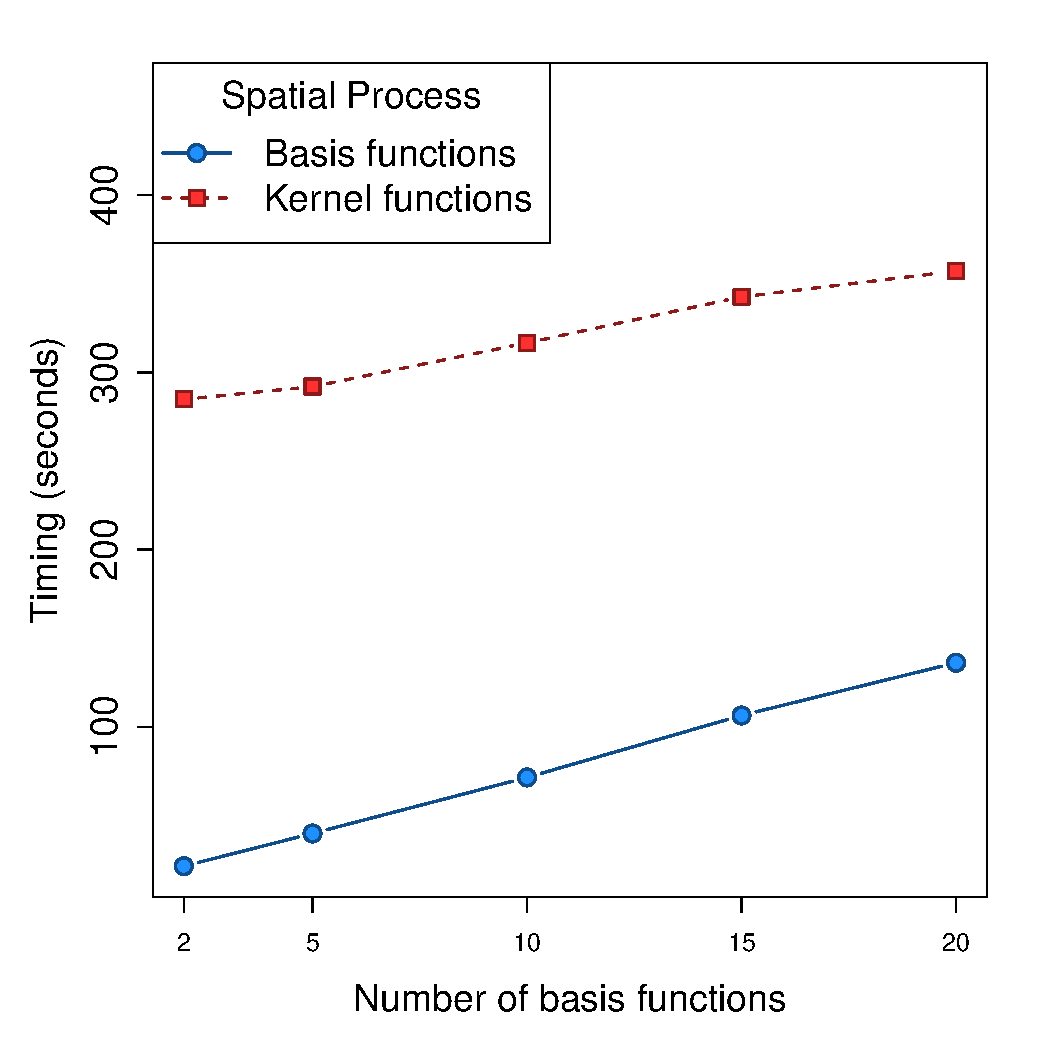
\includegraphics[width=0.47\linewidth]{plots/timing}
	\caption{Timing comparison of basis functions to kernel functions for the spatial process (100 iterations)}
  \label{fig:timingcompare}
\end{figure}

Based upon the cross-validation results, we reran the full data analysis using $L = 15$ basis functions.



\subsection{Model checking and sensitivity analysis}


\section{Conclusions}\label{s:con}

\section*{Acknowledgements}

\section*{A.1 Extreme value distributions}
Define (1) GEV density f and CDF F; (2) PS pdf  and the grid approximation to the integral.

\begin{singlespace}
\bibliographystyle{rss}
\bibliography{PCAX}
\end{singlespace}

\end{document}




